\section{The Compact Muon Solenoid experiment}
% intro

CMS uses a right-handed coordinate system centered on the nominal collision point with positive $x$ direction pointing towards the center of the LHC ring and the positive $y$ direction pointing vertically upward. The azimuthal angle in the $x$-$y$ plane, denoted $\phi$, is measured from the positive $x$ axis, and the polar angle $\theta$ is measured from the positive $z$ axis. The angle from the $z$ axis is more commonly described in terms of the pseudorapidity $\eta$, which is defined as $\eta=-\ln\tan(\theta/2)$ \cite{cms_tdr_v1}.

The CMS detector has undergone several upgrades since its initial construction. The description here will focus on the detector conditions relevant to the analysis presented in Section~\ref{displaced_leptons}.

\subsection{Solenoid magnet}
The superconducting solenoid responsible for the 'S' in CMS is designed to produce a \SI{4}{\tesla} magnetic field throughout the \SI{6.3}{\metre} diameter, \SI{12.5}{\metre} long cylindrical volume  that contains the CMS tracker and calorimeters. The magnetic field is produced by running \SI{19}{\kA} through 2168 turns of NbTi superconducting cable that are cooled with liquid helium. The flux returns through an iron yoke that also houses the muon system \cite{cms_experiment}. The strong magnetic field is critical to CMS's ability to unambiguously distinguish muons and anti-muons with transverse momenta up to \SI{1}{\TeV} \cite{cms_tdr_v1}.
% probably good to elaborate on physics importance

\subsection{Tracker}
\label{tracker}
In the region closest to the proton collisions, CMS employs a high-granularity silicon tracker to reconstruct particle trajectories and identify primary and secondary vertices. The tracker has a length of \SI{5.8}{\m}, a diameter of \SI{2.5}{\m}, and is composed of two subdetectors. Inside \SI{20}{\cm} from the beamline, the large particle flux demands the use of silicon pixel detectors, while silicon micro-strip detectors suffice in the region beyond \SI{20}{\cm} \cite{cms_experiment}. The original pixel detector was replaced between the 2016 and 2017 data-taking periods in preparation for higher luminosities \cite{cms_phase1_pixels}. As the analysis presented in Section~\ref{displaced_leptons} uses data collected in 2016--2018 and is particularly dependent on tracker measurements, the original pixel detector, 2017--2018 (Phase-1) pixel detector, and strip detector are described separately below. 

% \FIXME describe general detection mechanism and charge sharing and such

\subsubsection{Original pixel detector}
The original CMS pixel detector covers the $|\eta|<2.5$ region and is composed of three cylindrical barrel layers at $r=4.4$, $7.3$, and \SI{10.2}{\cm} and four endcap disks \num{34.5} and \SI{46.5}{\cm} up and down the beamline from the nominal collision point. Each layer or disk is instrumented with several pixel modules that are composed of a silicon sensor bump bonded to custom ASIC read-out chips (ROCs). Each sensor is \SI{285}{\um} thick and typically comprises 66560 $100\times\SI{150}{\um}$ pixels. The nearly square pixel shape enables approximately \SI{15}{\um} hit resolution in both the $r-\phi$ and $z$ directions \cite{cms_tdr_v1, cms_experiment}.

The original pixel detector was designed for a maximum instantaneous luminosity of \SI{e34}{\cm\tothe{-2}\s\tothe{-1}}, which corresponds to approximately 25 pileup collisions per bunch crossing at the LHC.

%  \FIXME: describe sensors and readout

\subsubsection{Phase-1 pixel detector}
The Phase-1 pixel detector represents an incremental improvement over the original CMS pixel detector: the same fundamental technology fills the same physical footprint and reuses many of the existing services but nevertheless achieves higher rate capabilities, improved radiation tolerance, and more robust tracking \cite{cms_phase1_pixels}. This is achieved by adding one additional layer to the barrel and each endcap, decreasing the radius of the innermost barrel layer to \SI{2.9}{\cm}, upgrading the ROCs, and reducing the material budget of the cooling system and mechanical structure \cite{cms_phase1_pixels, cms_phase1_pixel_tdr}. Figure~\ref{pixels_original_vs_phase1} compares the geometries of the original and Phase-1 pixel detectors.

% \FIXME: describe performance difference

\subsubsection{Strip tracker}
The strip tracker surrounds the pixel detector with silicon micro-strip sensors in 10 cylindrical barrel layers between $r=\SI{20}{\cm}$ and $r=\SI{110}{\cm}$ and 12 disks on each side of the barrel detector that extend to $|z|<\SI{282}{\cm}$ and cover up to $|\eta|<2.5$. The strip pitch generally increases with radius and results in hit resolutions that vary from \num{23} to \SI{530}{\um} \cite{cms_experiment}. Figure~\ref{tracker_layout} shows the layout of the entire silicon tracker.

\begin{figure}
\centering
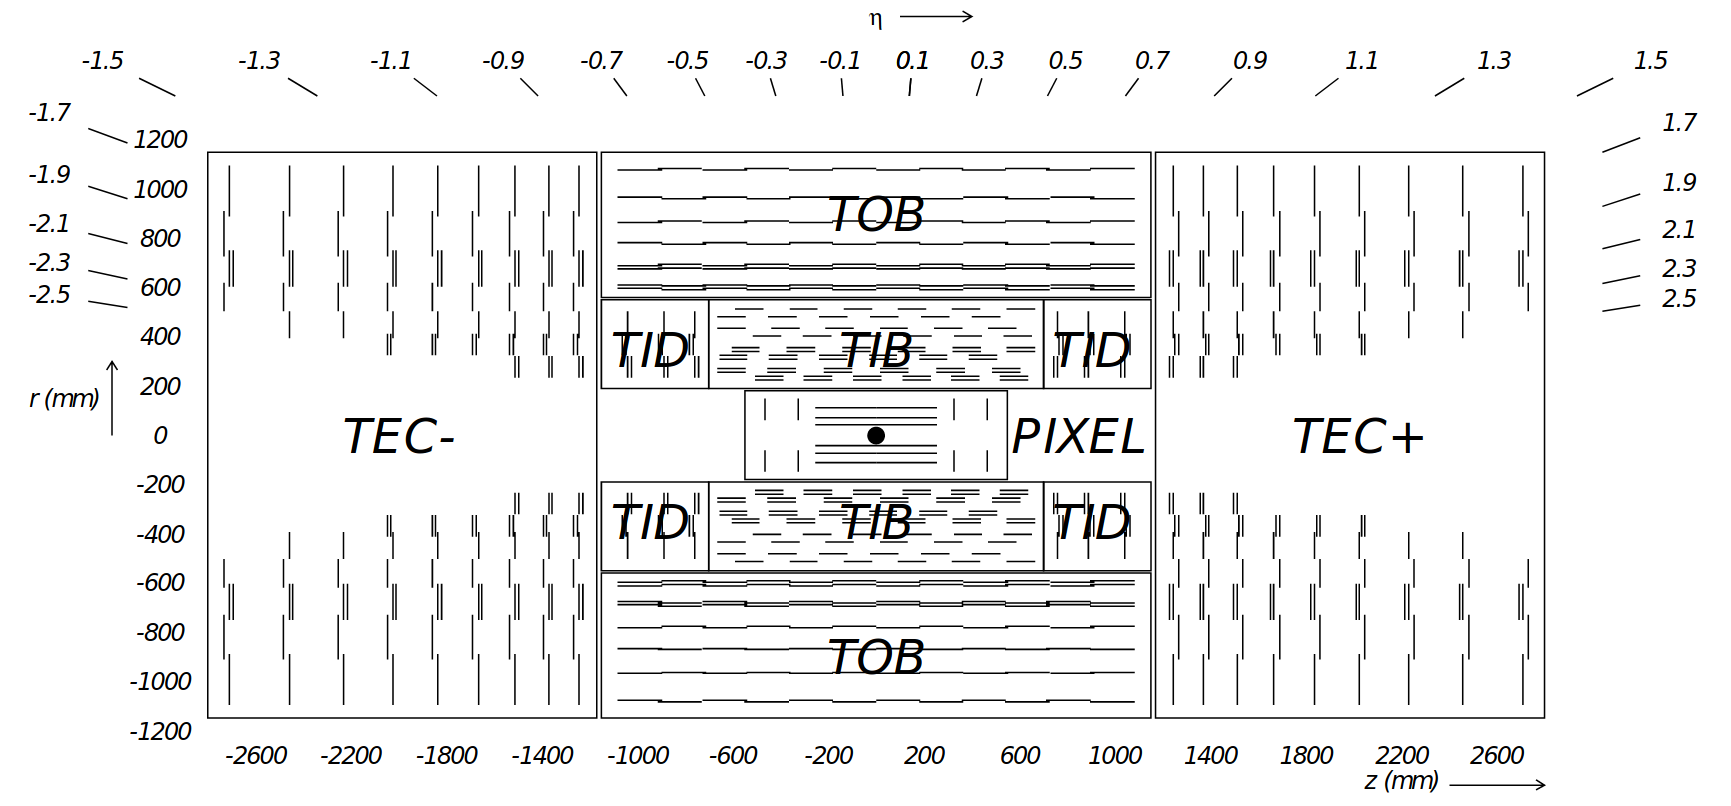
\includegraphics[width=\textwidth]{figures/lhc_and_cms/tracker_layout.png}
\caption{Layout of the CMS silicon tracker. TIB, TOB, TID, and TEC refer to subdetectors of the strip detector while PIXEL refers to the original pixel detector. The Phase-1 pixel detector is contained within the same volume~\cite{cms_experiment}.}
\label{tracker_layout}
\end{figure}

\begin{figure}
\centering
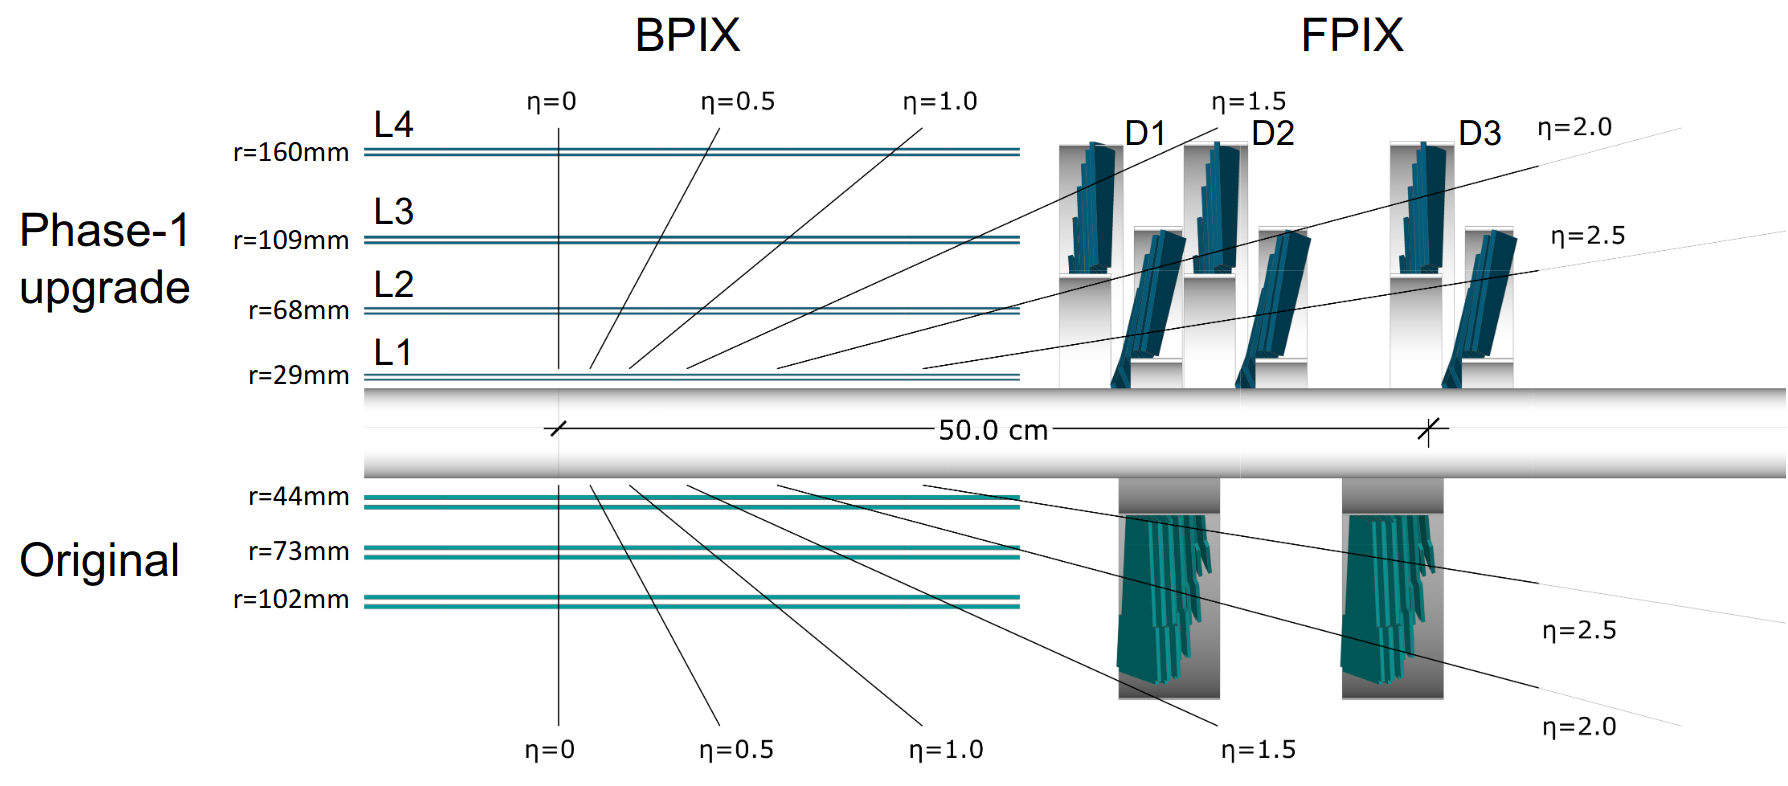
\includegraphics[width=0.9\textwidth]{figures/lhc_and_cms/pixels_layout_comparison.png}
\caption{Comparison of the original and Phase-1 CMS pixel detector layouts in $y$-$z$ plane~\cite{cms_phase1_pixels}.}
\label{pixels_original_vs_phase1}
\end{figure}

\subsection{Electromagnetic calorimeter}
After traversing the inner tracker, particles next encounter the electromagnetic calorimeter (ECAL). As a homogeneous scintillation calorimeter, ECAL uses \num{61200} lead tungstate crystals in the barrel and \num{7324} in each endcap to reconstruct the energy deposited during electromagnetic showers. Lead tungstate crystals allow for a fast (\SI{80}{\percent} of light emitted within \SI{25}{\ns}), compact (radiation length = \SI{0.89}{cm}), fine-grained (Moli\`ere radius = \SI{2.2}{\cm}), and radiation hard (up to \SI{10}{\mega rad}) calorimeter. The main drawback is the relatively low light yield (\SI{30}{photon\per\mega\electronvolt}), which necessitates photodetectors with intrinsic gain that work in magnetic fields\cite{cms_experiment, cms_tdr_v1}. Electron energy resolution varies from approximately \num{1}-\SI{5}{\percent} depending on the amount of material traversed before reaching ECAL~\cite{cms_ecal_performance}.

The barrel section extends radially from \num{129} to \SI{177}{cm} and covers up to $|\eta|<1.479$. The crystals are tapered to approximately project back to the IP but not so perfectly that likely particle trajectories align with cracks. Each crystal is approximately one Moli\`ere radius wide and 25 radiation lengths deep. The crystals in each endcap section are arranged in an x-y grid that starts at $\lvert z \rvert = \SI{315}{cm}$ and covers $1.479<\eta<3.0$.

\subsection{Hadronic calorimeter}
Particles that survive the ECAL will next encounter the hadronic calorimeter (HCAL). As the ECAL constitutes approximately 25 radiation lengths but only one interaction length, only particles that decay through the strong force will make it to the HCAL. HCAL is a sampling calorimeter that uses \SI{3.7}{\milli\metre} thick plates of plastic scintillator interspersed within brass absorber to reconstruct the energy deposited during hadronic showers. Embedded wavelength-shifting fibers capture the scintillation light and transfer it to clear fibers to be read out by hybrid photodiodes.

The barrel section ($|\eta|<1.4$) is segmented into \num{32} towers in $\eta$ and \num{64} in $\phi$ that each contain 17 active scintillator layers. In addition, an extra layer (or two at $\eta = \num{0}$) of scintillator tiles sits just outside the solenoid. This extra layer spans covers $|\eta<1.26|$ and increases the minimum effective HCAL interaction length to greater than \num{11.8}.

Each endcap spans a pseudorapidity range of \num{1.3} to \num{3.0} with \num{14} towers in eta and \num{5} to \SI{10}{\degree} $\phi$ segmentation. Also, a steel and quartz fiber forward calorimeter (HF) sits \SI{11.2}{m} from the interaction point and covers $3<|\eta|<5$. In HF, particles produce Cherenkov light when traversing the quartz fibers that run parallel to the beamline.


\subsection{Muon system}
The CMS muon system is composed of three varieties of gaseous detectors embedded in the iron return yoke outside the superconducting solenoid. In the central region ($|\eta|<1.2$), the low muon and neutron rates along with the lower magnetic field, allow the use of drift tube (DT) chambers. At higher $\eta$ ($0.9\leq|\eta|<2.4$), cathode strip chambers (CSCs) are required to handle the higher rates and larger magnetic field. Finally, resistive plate chambers (RPCs), which provide more accurate time measurements and worse spatial resolution than the DTs and CSCs, complement the other detectors out to $|\eta|<1.9$ \cite{cms_tdr_v1, cms_ms_performance}. 

\subsection{Trigger}
\label{trigger}
The trigger reduces the data writing rate from the \SI{40}{\MHz} collision rate to less than \SI{1}{\kHz} so that events can be written to tape. The rate reduction happens in two stages: Level-1 (L1) and High-Level Trigger (HLT). L1 analyzes input from ECAL, HCAL, and the muon system with custom electronics to reduce the rate to approximately \SI{100}{\kHz} in \SI{3.8}{\us}. With input from all subdetectors, the HLT then uses a dedicated processor farm to further reduce the rate to the desired $<$ 1 kHz\cite{cms_experiment, cms_trigger_upgrade}.

\subsection{Physics object reconstruction}
CMS uses a particle-flow (PF) algorithm to reconstruct the properties of individual particles by combining measurements from all subdetectors. Starting from charged particle tracks from the tracker and muon system and clusters of energy deposited in the ECAL and HCAL, CMS's PF algorithm aims to reconstruct all final-state electrons, muons, photons, and charged and neutral hadrons in a given event. This section first describes the reconstruction of tracks and energy clusters before moving on to individual particle identification and reconstruction. \cite{cms_pf} is cited throughout.

\subsubsection{Charged particle tracks}
Charged particle tracks are reconstructed with an iterative procedure. Despite the middling reconstruction efficiency of each individual step, starting with the highest-purity algorithms and masking the hits associated with each reconstructed track before moving on to the next step results in higher efficiency than could be achieved with any single tracking algorithm without increasing the rate of misreconstruction. This general principle applies to all charged particle tracks, but the tracks associated with candidate electrons and muons receive special consideration.

To better handle electron trajectories affected by radiative energy loss, CMS employs a special iterative tracking procedure that includes a Gaussian-sum filter (GSF) \cite{gsf}. This approach improves the overall reconstruction efficiency, allows reconstruction of lower-pT electrons, helps identify electrons from photon conversions, and helps distinguish electrons from charged hadrons.

Muon track reconstruction benefits from measurements in the tracker and the muon system. Candidate muon tracks are placed in one of three categories depending on which subdetectors are used in their reconstruction: \textit{standalone muon} tracks only use muon system hits, \textit{tracker muon} tracks only use tracker hits and the requirement of at least one consistent muon system hit, and \textit{global muon} tracks are reconstructed from a global fit of tracker and muon system hits.

\subsubsection{Calorimeter energy clusters}
Energy deposits in the calorimeters are clustered separately in ECAL and HCAL with a Gaussian-mixture model that assumes the energy deposits arise from an arbitrary number of Gaussian energy deposits whose amplitude and location are allowed to vary while the width is determined by the calorimeter properties. The clusters are first seeded by cells with energy above some threshold and greater than the energy of the surrounding cells. Nearby clusters are then merged before being fed to the Gaussian-mixture algorithm. Finally, several corrections are applied to the cluster energies to ensure accurate responses to photons and hadrons.

\subsubsection{Particle-flow reconstruction}
The tracks and clusters are then identified with and used to reconstruct all individual particles in an event. The first step is to link tracks and clusters together into groups that correspond one or a few particles. Tracker tracks are extrapolated outwards and linked with the nearest ECAL and HCAL clusters that within a set radius in the $\eta-\phi$ plane. In the case of candidate electron tracks, tracker tracks and ECAL deposits consistent with electron radiative losses are also linked with the candidate electron track. ECAL and HCAL clusters are similarly linked together by proximity in the $\eta-\phi$ plane. Due to the high granularity of CMS subdetectors, the number of tracks and clusters in a linked group is largely independent of the total number of particles in an event.

Each group of linked tracks and clusters is then processed by the PF particle identification and reconstruction algorithm. As in track reconstruction, particle reconstruction is an iterative process in which the tracks and clusters are masked after being associated with a particle. Figure~\ref{cms_slice} diagrams the basic concept used to identify muons, electrons, photons, and charged and neutral hadrons, and each step of the PF algorithm is summarized below.

Muons are reconstructed first from isolated \textit{global muon} candidates, then non-isolated \textit{global muon} candidates, and finally \textit{tracker muon} (\textit{standalone muon}) candidate tracks that are particularly well measured and consistent with hits in the muon system (tracker). Muon momentum is taken from the tracker track when $\pt<\SI{200}{\GeV}$ and from the combination of tracker and muon system hits yields the best fit otherwise.

Electrons and isolated photon reconstruction, which occur together after muon reconstruction, are necessarily interrelated by the high probability that an electron radiates a photon or a photon pair-produces electrons when interacting with tracker material. Electrons are identified from GSF tracks with a corresponding ECAL cluster while isolated photons are identified from isolated ECAL clusters. The total electron energy accounts for radiative losses that show up as ECAL clusters, and both electrons and isolated photons require a high ratio of ECAL cluster energy to nearby HCAL cluster energy.

Next, nonisolated photons and charged and neutral hadrons are reconstructed from the remaining tracks and clusters. Within the tracker acceptance ($|\eta|<2.5$), ECAL (HCAL) clusters without associated tracks are identified as photons (neutral hadrons). At higher $\eta$, nearby ECAL and HCAL clusters are assumed to arise from the same hadron shower and ECAL clusters without nearby HCAL clusters are identified as photons. Discrepancies between track momenta and associated HCAL cluster energy are also used to identify neutral hadrons and muons. Finally, a post-processing step corrects for rare failure modes that can potentially produce inaccurately large missing momentum.

%\subsubsection{Derived quantities and common variables}
%met, d0

\begin{figure}
\centering
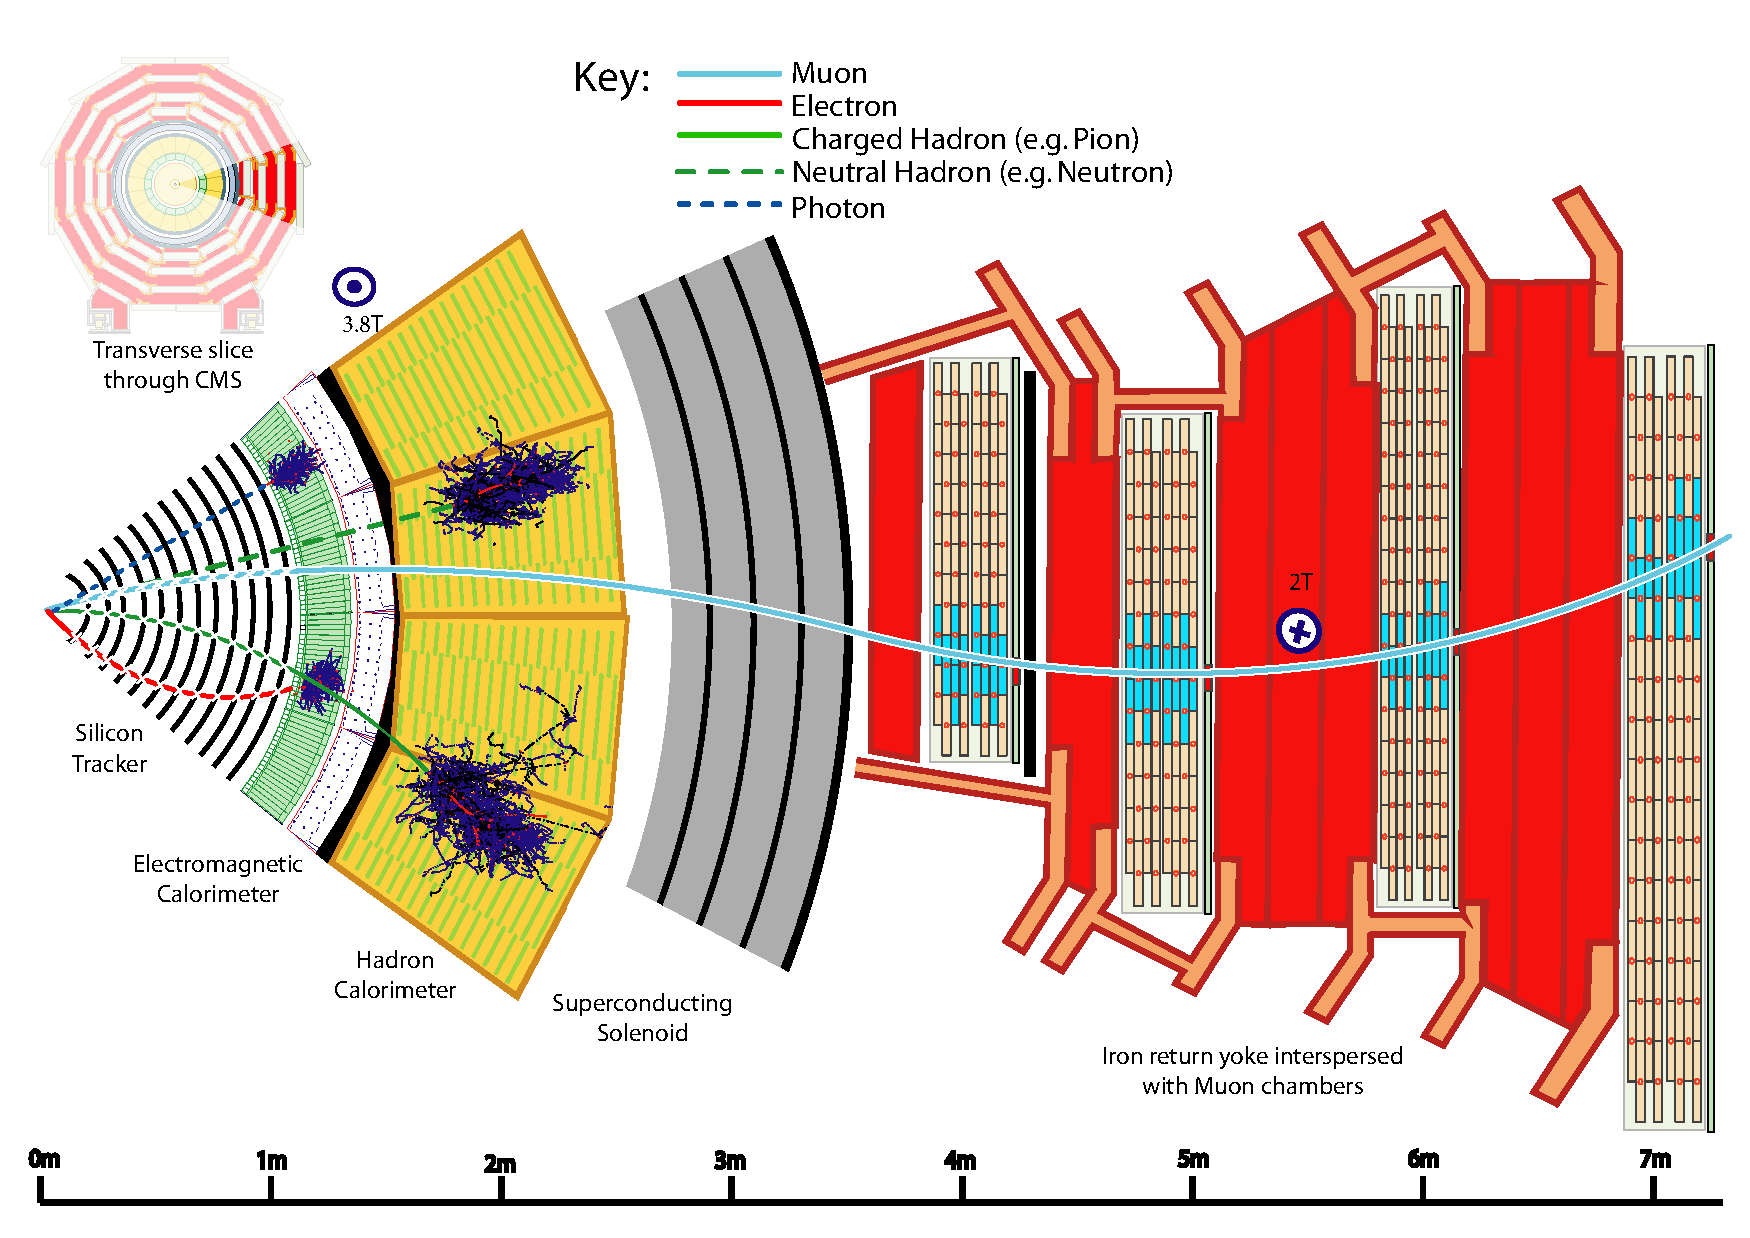
\includegraphics[width=\textwidth]{figures/lhc_and_cms/cms_slice.pdf}
\caption{A sketch of a transverse slice of the CMS detector showing representative particle interactions used to identify and reconstruct particles with the CMS Particle Flow algorithm \cite{cms_pf}.}
\label{cms_slice}
\end{figure}